\chapter{Introduction to Cataclysmic Variables}

% This chapter describes cataclysmic variable stars and their subset to which EC2117-54 belongs. It then describes the known properties of EC2117-54 derived from previous studies of the object. It concludes with a description of the aims of this project.

\section{Definition of Cataclysmic Variables}

Cataclysmic variables are semi-detached binary stars comprised of a white dwarf and a main sequence or an evolved star. The white dwarf star is usually called the primary and the companion star the secondary. The separation between the stars is small enough to cause the secondary to fill its Roche-lobe and donate its material through the inner lagrangian (L1) point to the primary star. Figure \ref{roche} shows a contour plot of the gravitational potentials of a binary system with $M_{1}=0.5M_{\odot}$, $M_{2}=0.125M_{\odot}$;  a mass ratio of $q = 0.25$ (where $q = \frac{M_{2}}{M_{1}}$) and an orbital period of 4 hours. The Roche-lobe is the equipotential that contains the L1 point, where the net gravitational force is zero. When mass transfer starts, the infalling material cannot fall directly onto the white dwarf. The stream of material initially follows a trajectory around the white dwarf and collides with itself. This collision process leads to a build-up of material and therefore  to the creation of an accretion disk around the primary, ultimately resulting in the material accreting onto the surface of the primary.

\begin{figure}
 \centering
 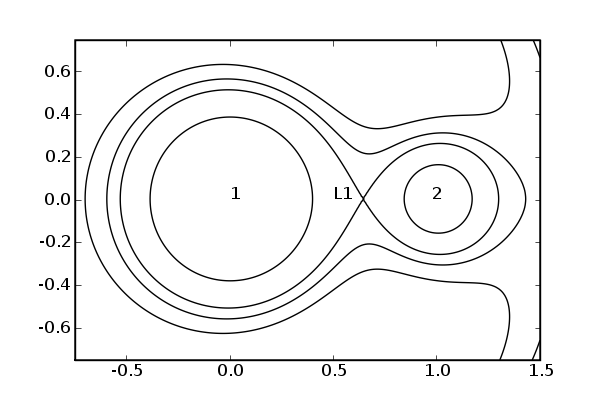
\includegraphics[width=0.85\columnwidth,bb=0 0 600 400]{images/roche.png}
 % roche.png: 600x400 pixel, 72dpi, 21.17x14.11 cm, bb=0 0 600 400
 \caption[Plot of Roche surface]{Plot of the Roche surfaces for a system with $\frac{M_{2}}{M_{1}}  = 0.25$ and $P = 4$ hours. The axes are labelled in units of binary separation. The labels ``1'' and ``2'' indicates positions of the white dwarf and red dwarf stars respectively.}
 \label{roche}
\end{figure}


\section{Formation of Cataclysmic Variables}


Cataclysmic variable stars are thought to form from a binary system in which the one star is more massive than the other. The more massive star (primary) depletes its hydrogen storage and evolves to the red giant stage. This results in an expansion of the envelope of the primary, leading to a common-envelope stage where the outer layers of the now-expanded primary contains the orbit of the secondary star. The increased aerodynamic friction on the secondary star causes angular momentum to be transferred from the secondary star to the outer layers of the expanded primary. The increase in the angular momentum causes the ejection of the outer layers of the primary into the interstellar medium. This process happens relatively quickly and ends in a pre-cataclysmic variable system which consists of a main sequence secondary orbiting the hot core of the primary star (subdwarf). The system is now detached \citep{warnerbible}.

In order for the orbit to decay further, a different mechanism of angular momentum loss is needed. The most likely possibilities are magnetic braking and gravitational radiation. It has been shown that magnetic braking is a more efficient mechanism of angular momentum loss than gravitational radiation for this stage of evolution of these stars and is therefore the mechanism driving angular momentum loss at this stage \citep{magbrake}.

Main sequence stars have solar winds consisting of particles being ejected at supersonic velocities. These particles are charged and must move along the star's magnetic field lines. Since the secondary star is rotating, the field lines are forced to rotate with it. The particles on the field lines provide a torque on the secondary star, opposing the rotation. This causes angular momentum loss and a subsequent decay of the orbit. When the orbit has decayed sufficiently, the secondary will fill its Roche-lobe and mass transfer commences. The system is now a semi-detached binary with stable mass transfer.


\section{Evolution of Cataclysmic Variables}

Cataclysmic variables undergo evolutionary changes. The main mechanisms for the evolution are mass transfer, magnetic braking and gravitational radiation. A histogram of all known cataclysmic variables shows a significantly lower number of systems with orbital periods between $\sim$2 and $\sim$3 hours than systems outside this range \citep{baraffekolb}. This is called the period-gap. For systems above the period-gap, magnetic braking is the mechanism which causes the orbital period to decrease. For the systems below the period-gap the mechanism is gravitational radiation.

The evolution of the orbital period works as follows. Mass is transferred from the secondary to the primary, carrying angular momentum with it.  The orbital separation increases and the secondary star shrinks by an infinitesimal amount and gets out of contact with its Roche-lobe. However, magnetic braking causes a decrease in orbital separation in order to conserve angular momentum. The  secondary therefore moves into contact with its Roche-lobe again. This is a continuous process and results in stable mass transfer and a decrease of the orbital period.

The mass transfer causes the convective zone of the secondary to become deeper over time. It is thought that at orbital periods of $\sim$3 hours, the convective core becomes deep enough to cause a sharp decrease in the solar wind outflow. The result is a sharp decrease in the mass transfer rate, because magnetic braking is no longer responsible for the angular momentum transfer \citep{warnerbible}. This is the so-called disrupted magnetic braking model \citep{baraffekolb}. At this stage the dominant mechanism for angular momentum transfer is gravitational radiation which becomes more efficient at lower orbital periods. At orbital periods of $\sim$2 hours, the secondary star moves into contact with its Roche-lobe and mass transfer can commence. The mass transfer rate is now lower than before the system evolved into the period-gap because gravitational radiation is less efficient at transferring angular momentum than magnetic braking.


%#########################################################
% Finish this!
% 
% 
% The angular momentum loss mechanism is still poorly understood. Recent studies show the evolution for systems below the perithe disrupted magnetic braking model 

%#########################################################


There is an observed period-minimum in the population of dwarf novae. This can be explained by evolution of the secondary to a point where it becomes semi-degenerate. Gravitational radiation causes the orbital period to decrease in the same manner as before. At an orbital period of $\sim$80 minutes, the secondary star has lost enough mass to become semi-degenerate. At this point, the orbital period starts to increase. As mass is transferred to the primary, the orbital separation increases. However, the volume of a semi-degenerate star increases slightly if mass is removed from it. This causes the secondary to fill its Roche-lobe at this increased orbital separation. The process is continuous and results in an increase in orbital period.



\section{Dwarf Nova Outbursts and Nova-likes }

\subsection{Disk Instability and Outbursts}

Long term monitoring of cataclysmic variables have shown systems that repeatedly undergo phases where the brightness of the system increases by up to 5 magnitudes. The most famous example of such a system is SS Cygni \citep{SSCyg}. These are dwarf nova outbursts and are thought to be the result of an instability in the accretion disk. 

The material transferred from the secondary builds up in the accretion disk and some of the material accretes onto the primary. The build-up of material causes the density of the disk to increase over time. This increase in density leads to an increase in the viscosity. Because viscosity is the mechanism which drives mass transfer through the disk, increased viscosity will increase the mass transfer through the disk. Material falling into a gravitational well such as this will radiate its energy away, thereby increasing the disk temperature. When the disk reaches $\approx 10000$ K the ionization of hydrogen causes the disk to become optically thick and absorb photons very efficiently. This causes a runaway reaction whereby the disk becomes fully ionized. The mass transfer rate will now commence at a high rate and dump a large amount of material onto the white dwarf. However, the rate of cooling in this `high-state' disk exceeds the rate of heating and the disk will gradually cool off. When it reaches the point where hydrogen can recombine, the disk starts cooling rapidly and returns to its quiescent state. 



\subsection{Nova-like Variables}
\label{novalikes}

A different scenario is possible for the state of the accretion disk. If the mass transfer rate is high enough, the disk can be permanently held in a high state i.e. the system is in permanent outburst. These systems are called nova-like (NL) variables. An example of such as system is V348 Puppis \citep{v348pup}. They generally have orbital periods between 3 and 4 hours. These stars have a relatively constant brightness and do not show outbursts like the dwarf novae.

The accepted classification of NLs are given in \cite{dhillon_NL} and \cite{warnerbible}. The NL systems that are not classified as magnetic systems are the UX Ursae Majoris (UX UMa) stars and the RW Tri stars. They show absorption and emission lines, respectively. See \cite{Knigge_HST_UX_UMa} for a study of the UX UMa prototype star. Some UX UMa stars enter states of low brightness. These  systems are called the VY Scl stars. Some UX UMa and VY Scl with high inclinations are observed with single-peaked emission lines and are classified as SW Sex stars. See \cite{swsex} for a discussion on the nature of SW Sex.


\section{Rapid Oscillations in Cataclysmic Variables}

The accretion process in cataclysmic variable stars is a rich source of variability in the brightness of these stars. The observation of flickering in the lightcurve of a stellar object is a tell-tale sign of accretion. Apart from the flickering, orbital modulation and eclipses observed in many examples of these stars, other stable signals can also be detected. In 1954, Merle Walker discovered the first coherent signal on a very short timescale in the object DQ Her \citep{dqher}.

There are three different stable rapid oscillations observed in dwarf novae during outburst, as well as in nova-like variables. These are the Dwarf Nova Oscillations (DNO), long period DNOs (lpDNO) and the Quasi-Periodic Oscillations (QPO)\citep{warner_ro2004}. Their stability is measured using the parameter $Q = \vert \dot{P}^{-1} \vert$.  $\dot{P}$ is the rate at which the period ($P$) changes.  The 71s period of DQ Her has a $ Q >  10^{12} $ \citep{warnerbible} and is associated with the spin period of the white dwarf. 

DNOs are rapid oscillations with periods generally of the order of tens of seconds. They are observed during outburst in dwarf novae as well as in nova-like variables and are sometimes stable to milliseconds over several hours, or can change their period by a few seconds in a few hours but generally have $ 10^{4} \lesssim Q \lesssim 10^{6} $ in the optical (or less for X-ray) observations \citep{warner_ro2004}. They generally have an amplitude of a few to a few tens of millimagnitudes. The current accepted, albeit untested, model for DNOs involves mass accretion onto a slipping equatorial belt on the white dwarf primary. The model is very similar to that of the Intermediate Polar (IP) model which involves a magnetically truncated accretion disk near the primary. The material moving through the disk gets threaded onto field lines near the white dwarf and accretes onto the magnetic poles of the primary \citep{warnerbible}. In the case of the Low-Inertia Magnetic Accretor (LIMA) \citep{DNOQPO_II} model for DNOs, the accretion onto the white dwarf is controlled by the magnetic field only very close to the white dwarf. The reasoning is that during quiescent states in dwarf novae with weaker fields, the magnetic field is too weak to force the star to rotate as a solid body. However, in the times of increased mass transfer during outburst, the material accretes onto the equator of the white dwarf thereby increasing the rotational velocity of this band on the star and causing it to slip. This causes a shear in the magnetic fields that are contained within this region, causing the field to increase in strength \citep{DNOQPO_II} and start enforcing magnetic accretion. This model requires the white dwarf to have a magnetic field of less than about $10^{5}$ Gauss. \cite{DNOQPO_II} also argues that the abrupt frequency changes seen in DNOs is caused by the snapping and reconnection of magnetic field lines along the rotating equatorial belt.

Oscillations with a similar timescale of stability as the DNOs but with a longer period by about a factor of 4 are the lpDNOs. See \cite{warner_ro2004} and \cite{WWP}. They can co-exist with the DNOs. Different models exist to explain the behaviour of lpDNOs and have been described in \cite{DNOQPO_VI}.

QPOs are oscillations with a much lower coherence ($Q \sim 10 $) than that of DNOs and lpDNOs \citep{WWP}. They are usually seen at periods of $\approx 15$ times the DNO period. Their low coherence makes it difficult to identify QPOs using Fourier techniques because their power is spread over a range of frequencies \citep{warner_ro2004}. It is thought that there may be several types of QPOs observed in CVs. In some stars double DNOs are observed where the beat period between the DNOs is approximately equal to the QPO period. The QPOs are thought to be caused by a progradely travelling wave in the inner parts of the accretion disk \citep{warner_ro2004}, thereby causing modulation of the lightcurve by obscuring or reprocessing light from the central source. The wave can be seen as a thickening of the accretion disk. QPOs without any obvious relation to the DNOs are also sometimes observed. These may have periods similar to the rotation period of the outer parts of high $\dot{M}$ (high mass-transfer rate) disks. The study of QPOs is made difficult by their low coherence and the inherent flickering of the accretion disk.  For an in-depth review of rapid oscillations in cataclysmic variables see \cite{warner_ro2004}.
 

\section{EC2117-54}
\label{ec2117}

EC2117-54 is a nova-like cataclysmic variable with V $\sim13.7$. It was found as an emission line object in the Edinburgh-Cape survey of blue objects in the southern hemisphere \citep{ecsurvey}. It has an orbital period of $\sim3.708$ hours and shows deep V-shaped eclipses. Spectroscopy reveals double-peaked emission lines and therefore puts the system in the RW Tri category. 

It is also known to regularly show DNOs and lpDNOs \citep{WWP}. Since it is relatively bright and shows DNOs and lpDNOs $\sim80$\% of the time, it is a perfect candidate with which to study these rapid oscillations in detail using high-speed spectroscopic and photometric methods.



\section{Aim of the project}
\label{aim}

An area of research that only became possible in the last decade, with the advent of 10m class telescopes, 
is the study of short period variations in the observed emission line and continuum flux of astronomical objects. The objects with the fastest known periodicities are neutron stars and the interacting binary systems they occur in. Since these are usually very faint and have most of their flux in the X-ray regime, they are not suitable for high-speed spectroscopic studies from the ground. 

Similar systems, but with more favourable properties for optical spectroscopy are the cataclysmic variables. They provide the perfect testbed for the study of accretion disk physics, since a large number of them are relatively bright and easily observable with some of the world's largest optical and infrared telescopes. Cataclysmic variables are known to produce stable variations with very short periods (2-40s) \citep{warnerbible}. These objects provides us with a unique opportunity to study their intrinsic properties, as well as accretion disks in general, using high time-resolution spectroscopy.

The first generation instruments (SALTICAM and the Robert Stobie Spectrograph (RSS)) installed on the Southern African Large Telescope (hereafter SALT)  are both designed to produce exceptional high time-resolution observations. This is one of the foreseen niche areas of SALT (and South African astronomy). This project's focus is to study rapid oscillations in an eclipsing cataclysmic variable star using the high-speed capability of the RSS together with high-quality photometric observations using the South African Astronomical Observatory (SAAO) 1.9m telescope. In particular, the behaviour of DNOs and lpDNOs are to be studied during times of eclipse. This will give an indication of the location in the system where these oscillations originate. The spectroscopic observations were made during the performance verification (PV) phase  of SALT and as such the RSS was not yet working optimally.



This project aims to identify and analyse the short period variations that are observed in high-speed photometric studies of CVs, using time-resolved spectroscopic observations of EC2117-54 as an example. This is not an entirely unexplored avenue. Studies of this kind have been done in the past using the Low Resolution Imaging Spectrograph (LRIS) on the Keck II telescope. See \cite{V2051Oph2001} and \cite{AEAqu2003} for examples on V2051 Oph and AE Aquarii respectively.

The task is made difficult due to the varying aperture size and vignetting during SALT observations and some techniques must be developed and tested to overcome these difficulties. This study combines high-speed photometric and high-speed spectroscopic observations to achieve the desired results.




